\documentclass[11pt,twoside]{article}
\usepackage[utf8]{inputenc}
\usepackage[T1]{fontenc}

% Page margins, header and footer positions
\usepackage{geometry}
\geometry{
 a4paper,
 total={210mm,297mm},
 left=25mm,
 right=25mm,
 top=30mm,
 bottom=25mm,
 headsep=7mm
}

\interfootnotelinepenalty=10000

% To display filling dots in the TOC for all entries
\usepackage[titles]{tocloft}
\renewcommand{\cftsecleader}{\cftdotfill{\cftdotsep}}

% Define new header and footer style
\usepackage{fancyhdr}

\pagestyle{fancy}
\fancyhf{}
\lhead{\color{Gray}{\small{Travlendar+ project by YOUR NAMES}}}
\lfoot{\textcolor{Gray}{\small{Copyright © 2017, YOUR NAMES – All rights reserved}}}
\rfoot{\textcolor{Gray}{\thepage}}
\renewcommand{\headrulewidth}{0pt}

% PACKAGES
\usepackage{wasysym}
\usepackage{pifont}

\newcommand{\supported}{\ding{52}\xspace}
\newcommand{\unsupported}{\ding{55}\xspace}
\newcommand{\partsupported}{\textcolor{black!40}{\ding{52}}\xspace}
\newcommand{\lowsupported}{\textcolor{black!20}{\ding{52}}\xspace}
\newcommand{\unknowsupported}{\textbf{?}\xspace}

% Font: Times
\usepackage{times}
% Change monospaced font
\renewcommand{\ttdefault}{lmtt}

% Tables
\usepackage{tabu}
\usepackage{tabularx}
\usepackage{ltablex}
\usepackage{longtable}
\usepackage{float}

% Landscape mode
\usepackage{pdflscape}
\usepackage{rotating}
\usepackage{caption}

% Make landscape mode be sensitive to even and odd pages
\def\myrotate{\ifodd\c@page\else-\fi 90}
\makeatletter
\global\let\orig@begin@landscape=\landscape%
\global\let\orig@end@landscape=\endlandscape%
\gdef\@true{1}
\gdef\@false{0}
\gdef\landscape{%
    \global\let\within@landscape=\@true%
    \orig@begin@landscape%
}%
\gdef\endlandscape{%
    \orig@end@landscape%
    \global\let\within@landscape=\@false%
}%
\@ifpackageloaded{pdflscape}{%
    \gdef\pdf@landscape@rotate{\PLS@Rotate}%
}{
    \gdef\pdf@landscape@rotate#1{}%
}
\let\latex@outputpage\@outputpage
\def\@outputpage{
    \ifx\within@landscape\@true%
        \if@twoside%
            \ifodd\c@page%
                \gdef\LS@rot{\setbox\@outputbox\vbox{%
                    \pdf@landscape@rotate{-90}%
                    \hbox{\rotatebox{90}{\hbox{\rotatebox{180}{\box\@outputbox}}}}}%
                }%
            \else%
                \gdef\LS@rot{\setbox\@outputbox\vbox{%
                    \pdf@landscape@rotate{+90}%
                    \hbox{\rotatebox{90}{\hbox{\rotatebox{0}{\box\@outputbox}}}}}%
                }%
            \fi%
        \else%
            \gdef\LS@rot{\setbox\@outputbox\vbox{%
                \pdf@landscape@rotate{+90}%
                \hbox{\rotatebox{90}{\hbox{\rotatebox{0}{\box\@outputbox}}}}}%
            }%
        \fi%
    \fi%
    \latex@outputpage%
}
\makeatother

% Graphics
\usepackage{graphicx}
\usepackage[dvipsnames, table]{xcolor}

% Other
\usepackage{ifthen}
\usepackage{xspace}
\usepackage{enumitem}
\usepackage{amssymb}
\usepackage[pdftex, colorlinks]{hyperref}
\newcommand{\comment}[1]{{\color{Red}$\blacktriangleright$ Comment: #1 $\blacktriangleleft$}}

% Some utilities
\usepackage{soul}
\usepackage{tikz}

\usetikzlibrary{calc}
\usetikzlibrary{decorations.pathmorphing}


\makeatletter

\newcommand{\defhighlighter}[3][]{%
  \tikzset{every highlighter/.style={color=#2, fill opacity=#3, #1}}%
}

\defhighlighter{yellow}{.5}

\newcommand{\highlight@DoHighlight}{
  \fill [ decoration = {random steps, amplitude=1pt, segment length=15pt}
        , outer sep = -15pt, inner sep = 0pt, decorate
       , every highlighter, this highlighter ]
        ($(begin highlight)+(0,8pt)$) rectangle ($(end highlight)+(0,-3pt)$) ;
}

\newcommand{\highlight@BeginHighlight}{
  \coordinate (begin highlight) at (0,0) ;
}

\newcommand{\highlight@EndHighlight}{
  \coordinate (end highlight) at (0,0) ;
}

\newdimen\highlight@previous
\newdimen\highlight@current

\DeclareRobustCommand*\highlight[1][]{%
  \tikzset{this highlighter/.style={#1}}%
  \SOUL@setup
  %
  \def\SOUL@preamble{%
    \begin{tikzpicture}[overlay, remember picture]
      \highlight@BeginHighlight
      \highlight@EndHighlight
    \end{tikzpicture}%
  }%
  %
  \def\SOUL@postamble{%
    \begin{tikzpicture}[overlay, remember picture]
      \highlight@EndHighlight
      \highlight@DoHighlight
    \end{tikzpicture}%
  }%
  %
  \def\SOUL@everyhyphen{%
    \discretionary{%
      \SOUL@setkern\SOUL@hyphkern
      \SOUL@sethyphenchar
      \tikz[overlay, remember picture] \highlight@EndHighlight ;%
    }{%
    }{%
      \SOUL@setkern\SOUL@charkern
    }%
  }%
  %
  \def\SOUL@everyexhyphen##1{%
    \SOUL@setkern\SOUL@hyphkern
    \hbox{##1}%
    \discretionary{%
      \tikz[overlay, remember picture] \highlight@EndHighlight ;%
    }{%
    }{%
      \SOUL@setkern\SOUL@charkern
    }%
  }%
  %
  \def\SOUL@everysyllable{%
    \begin{tikzpicture}[overlay, remember picture]
      \path let \p0 = (begin highlight), \p1 = (0,0) in \pgfextra
        \global\highlight@previous=\y0
        \global\highlight@current =\y1
      \endpgfextra (0,0) ;
      \ifdim\highlight@current < \highlight@previous
        \highlight@DoHighlight
        \highlight@BeginHighlight
      \fi
    \end{tikzpicture}%
    \the\SOUL@syllable
    \tikz[overlay, remember picture] \highlight@EndHighlight ;%
  }%
  \SOUL@
}

\makeatother

% !TeX root = ../dd.tex
% Common abbrev. are set as commands to ensure proper spacing after the dot
\RequirePackage{xspace}
\newcommand{\ie}{i.e.\@\xspace}
\newcommand{\aka}{a.k.a.\@\xspace}
\newcommand{\Ie}{I.e.\@\xspace}
\newcommand{\cf}{cf.\@\xspace}
\newcommand{\Cf}{Cf.\@\xspace}
\newcommand{\eg}{e.g.\@\xspace}
\newcommand{\Eg}{E.g.\@\xspace}
\newcommand{\etal}{et al.\@\xspace}
\newcommand{\etc}{etc.\@\xspace}
\newcommand{\wrt}{w.r.t.\@\xspace}
\newcommand{\Wrt}{W.r.t.\@\xspace}

\begin{document}

% TITLE PAGE
\begin{titlepage}
% LOGO
{\begin{table}[t!]
\centering
\begin{tabu} to \textwidth { X[1.3,r,p] X[1.7,l,p] }
\textcolor{Blue}
{\textbf{\small{Travlendar+ project YOUR NAMES}}} & 
\includegraphics[scale=0.5]{Images/PolimiLogo}
\end{tabu}
\end{table}}~\\ [7cm]

% TITLE 
\begin{flushleft}
{\textcolor{Blue}{\textbf{\Huge{Requirement Analysis and Specification
        Document}}}} \\ [1cm]
\end{flushleft}
\end{titlepage}

% Define deliverable specific info
\begin{table}[h!]
\begin{tabu} to \textwidth { X[0.3,r,p] X[0.7,l,p] }
\hline
\textbf{Deliverable:} & RASD\\
\textbf{Title:} & Requirement Analysis and Verification Document \\
\textbf{Authors:} & YOUR NAMES \\
\textbf{Version:} & 1.0 \\ 
\textbf{Date:} & 31-January-2016 \\
\textbf{Download page:} & LINK TO YOUR REPOSITORY \\
\textbf{Copyright:} & Copyright © 2017, YOUR NAMES – All rights reserved \\
\hline
\end{tabu}
\end{table}

\setcounter{page}{2}

\newpage
\addcontentsline{toc}{section}{Table of Contents}
\tableofcontents
\newpage
\addcontentsline{toc}{section}{List of Figures}
\listoffigures
\addcontentsline{toc}{section}{List of Tables}
\listoftables

\clearpage
{\color{Blue}{\section{Introduction}}}
\label{sect:introduction}
\section{Purpose}
The purpose of the system Student\&Companies (S\&C) is to help matching university student who are looking for internship with companies that are offering them. The matching system is based on student's experiences, skills and attitude crossed with the projects and terms offered by the various companies. There are two ways in which students can get an internship, one is by being proactive and initiating the application process and the other one is by being recommended to a company by the platform.

The goals of the S\&C platform are:
\begin{enumerate}[label=\textbf{G\arabic*}:,ref=G\arabic*,leftmargin=1.3cm]
    \labelleditem{Students can list their experiences, skills and attitudes in their CVs}
    \labelleditem{Companies can post the projects students are going to work on during their internships (specifying topics, tasks and technologies adopted) with the relative compensations and benefits}
    \labelleditem{Students can initiate the process by going through the available internships}
    \labelleditem{Students can be notified when an internship that might interest them becomes available}
    \labelleditem{Companies can be notified about the availability of students CVs corresponding to their needs}
    \labelleditem{Students and companies can accept or decline a recommendation}
    \labelleditem{Companies can interview students}
    \labelleditem{Students and Companies can monitor the execution and the outcomes of the selection procedure}
    \labelleditem{Student can report on a logbook the daily situation of the internship}
    \labelleditem{Universities can monitor the situation of the internship}
    
\end{enumerate}

\pagebreak

\section{Scope}
Students that use the platform are enrolled in a university and are looking for an internship. Companies use the platform to advertise the internship they are offering. 

The platform integrates its login and registration process with an existing Single Sign-On (SSO) system, which handles user authentication.

The platform asks a series of questions to students that want to upload their CV. Once the student wants to contact a company the system will generate a personalized and editable CV, tailored on the company's requirements. Furthermore it helps companies to make project description more apprizing for students.

A personalized homepage will be created by the system for both students and companies based on the information they gave during the registration.

Students can be proactive when looking for an internship by going through the personalized list of available experiences but also can be notified by the system when an internship that might interest them becomes available. 

The system also notifies companies about the availability of student's CVs corresponding to their needs.

When these suggestions are accepted by the two parties, a contact is established. After a contact is settled a selection process starts.

During the process companies interview students to determine if the students will fit with the company and the internship. 

The system will also support the selection process by setting up, conduct and manage the interviews. At the end of the process it will also help finalizing the selections.

To collect data the system asks to students and companies to provide feedback or suggestions regarding the internships.

The system provides all interested parties with tools to track and monitor the execution and outcomes of the matchmaking process. It also provide spaces where interested parties can complain, communicate problems and provide information regarding the status of the ongoing internship.

Universities monitor the situation of internships, they are responsible for handling the complaints, especially when one of the two parties want to interrupt the internship.


The following table describes world, shared and machine phenomena.
\begin{center} %Limits the scope of \rowcolors
    \rowcolors{2}{gray!25}{white}
    \begin{longtable}{|p{8.7cm}|p{3cm}|p{3cm}|}
        \caption[Phenomena Table]{}
        \label{table:phenomena}
        \endlastfoot
        \hline
        \rowcolor{gray!50}
        \textbf{Phenomena}                                                                                                                & \textbf{Controlled by} & \textbf{Shared} \\ \hline
        A user wants to log in to the platform & W & N \\ \hline
        A company wants to create a new internship & W & N \\ \hline
        A student wants to insert information to create  his CV   & W  & N \\ \hline
        A student wants to look for an internship & W  & N \\ \hline
        The system creates the personalized CV  & M  & Y \\ \hline
        The system makes a suggestion to produce a more appealing project description  & M  & Y \\ \hline
        The system notifies a student when an internship that may interest him becomes available & M  & Y \\ \hline
        The system notifies a company when a student's CV corresponding their needs is available & M  & Y \\ \hline
        The system starts a selection process when two related suggestions are accepted by the two parties & M  & N \\ \hline
        The system supports the selection process by setting up, conducting and managing the interviews. & M  & Y \\ \hline
        At the end of the process the system will also help finalizing the selections & M  & Y 
        \\ \hline
        The system asks to a student to provide a feedback or a suggestion about the internship & M  & Y \\ \hline
        The system asks to a company to provide a feedback or a suggestion about the internship & M  & Y \\ \hline
        The system shows the current state of the matchmaking process & M  & Y \\ \hline
        Any user write in the "Report Area" section & W  & Y \\ \hline
        University handle a complaint & W  & Y \\ \hline
        Any user want to interrupt the internship & W  & N \\ \hline
    \end{longtable}
\end{center}
\pagebreak

\section{Definitions, Acronyms, Abbreviations}


\subsection{Definitions}
\begin{description}[leftmargin=0pt]
\item[Curriculum Vitae (CV):] A brief account of a person's education,  qualifications, and previous occupations, typically sent with a job application.
\item[Students\&Companies:] A platform designed to help students and businesses to find an internship.
\item[Single Sign On (SSO)]: A way to login into the system using the credentials offered by the University or the company. 
\item[Internship:] The position of a student or trainee who works in an organization, in order to gain work experience or satisfy requirements for a qualification.
\item[Recommendation:] The process of informing students and companies when an interesting internship becomes available or about the availability of a student CVs corresponding the needs of a company.
\item[Project:] set of tasks the company assign to their internee.
\item[Task:] a piece of work.
\item[Interviews:] A meeting between the student and the company where the student has to demonstrate to be fit for the company's internship. 
\item[Feedback:] Information about how the internship is going from both of the parties.
\item [Report Area:] A space where a student or a company can complain, communicate problems, and provide information about the current status of the ongoing internship.
\item[My CV:] Section of the website where the student is able to create his CV.

\end{description}


\subsection{Acronyms}
\begin{description}[leftmargin=0pt]
    \item [SSO:] Single Sign On
    \item [API:] Application Programming Interface
    \item [CV:] Curriculum Vitae
    \item [S\&C:] Students\&Companies
    \item [IDE:] Integrated Development Environment
\end{description}


\subsection{Abbreviations}
\begin{description}[leftmargin=0pt]
    \item[e.g.:] For example
    \item [w.r.t.:] With reference to
\end{description}

\section{Revision history}

\begin{itemize}
    \item 
\end{itemize}

\section{Reference Documents}
\begin{description}[leftmargin=0pt]
    \item[Specification document:] \emph{"Assignment RDD AY 2024-2025"}
    \item[UML official specification:] \url{https://www.omg.org/spec/UML/}
    \item[Alloy official documentation:] \url{https://alloytools.org/documentation.html}
\end{description}

\section{Document Structure}

\begin{enumerate}
    \item \textbf{Section 1: Introduction} \\
          This section exposes the purpose and the scope of the system explaining the goals of the project and including the analysis of the world and the shared phenomena. x  aq
          It also contains definitions acronyms and abbreviations to make sure the document is not ambiguous.
    \item \textbf{Section 2: Overall Description} \\
          This section contains an overall description about the product prospective including scenarios and detail on the shared phenomena and a domain model expressed through class diagram and state diagram. It also include the product functions with the most important requirements and categories of use cases. It also contains the assumptions, dependencies and constraints.
          
    \item \textbf{Section 3: Specific Requirements} \\
          This section describes the specific requirements, in particular there are details on all aspects that may be useful for the development team.
          It provides external interface requirements, which include user, hardware, software and communication interfaces.
          Finally, it describes performance and functional requirements, through the use of use case diagrams, use cases, related sequences, activity diagrams, and mapping on requirements.
    \item \textbf{Section 4: Formal Analysis using Alloy} \\
        This section provides a formal analysis using the alloy language with a brief presentation of the main objectives driving the formal modeling activity. This is done to prove the correctness and soundness of the system described in the previous sections.
\end{enumerate}


\clearpage
{\color{Blue}{\section{Overall Description}}}
\label{sect:overview}
Here you can see how to include an image in your document.

\begin{sidewaysfigure}
\centering
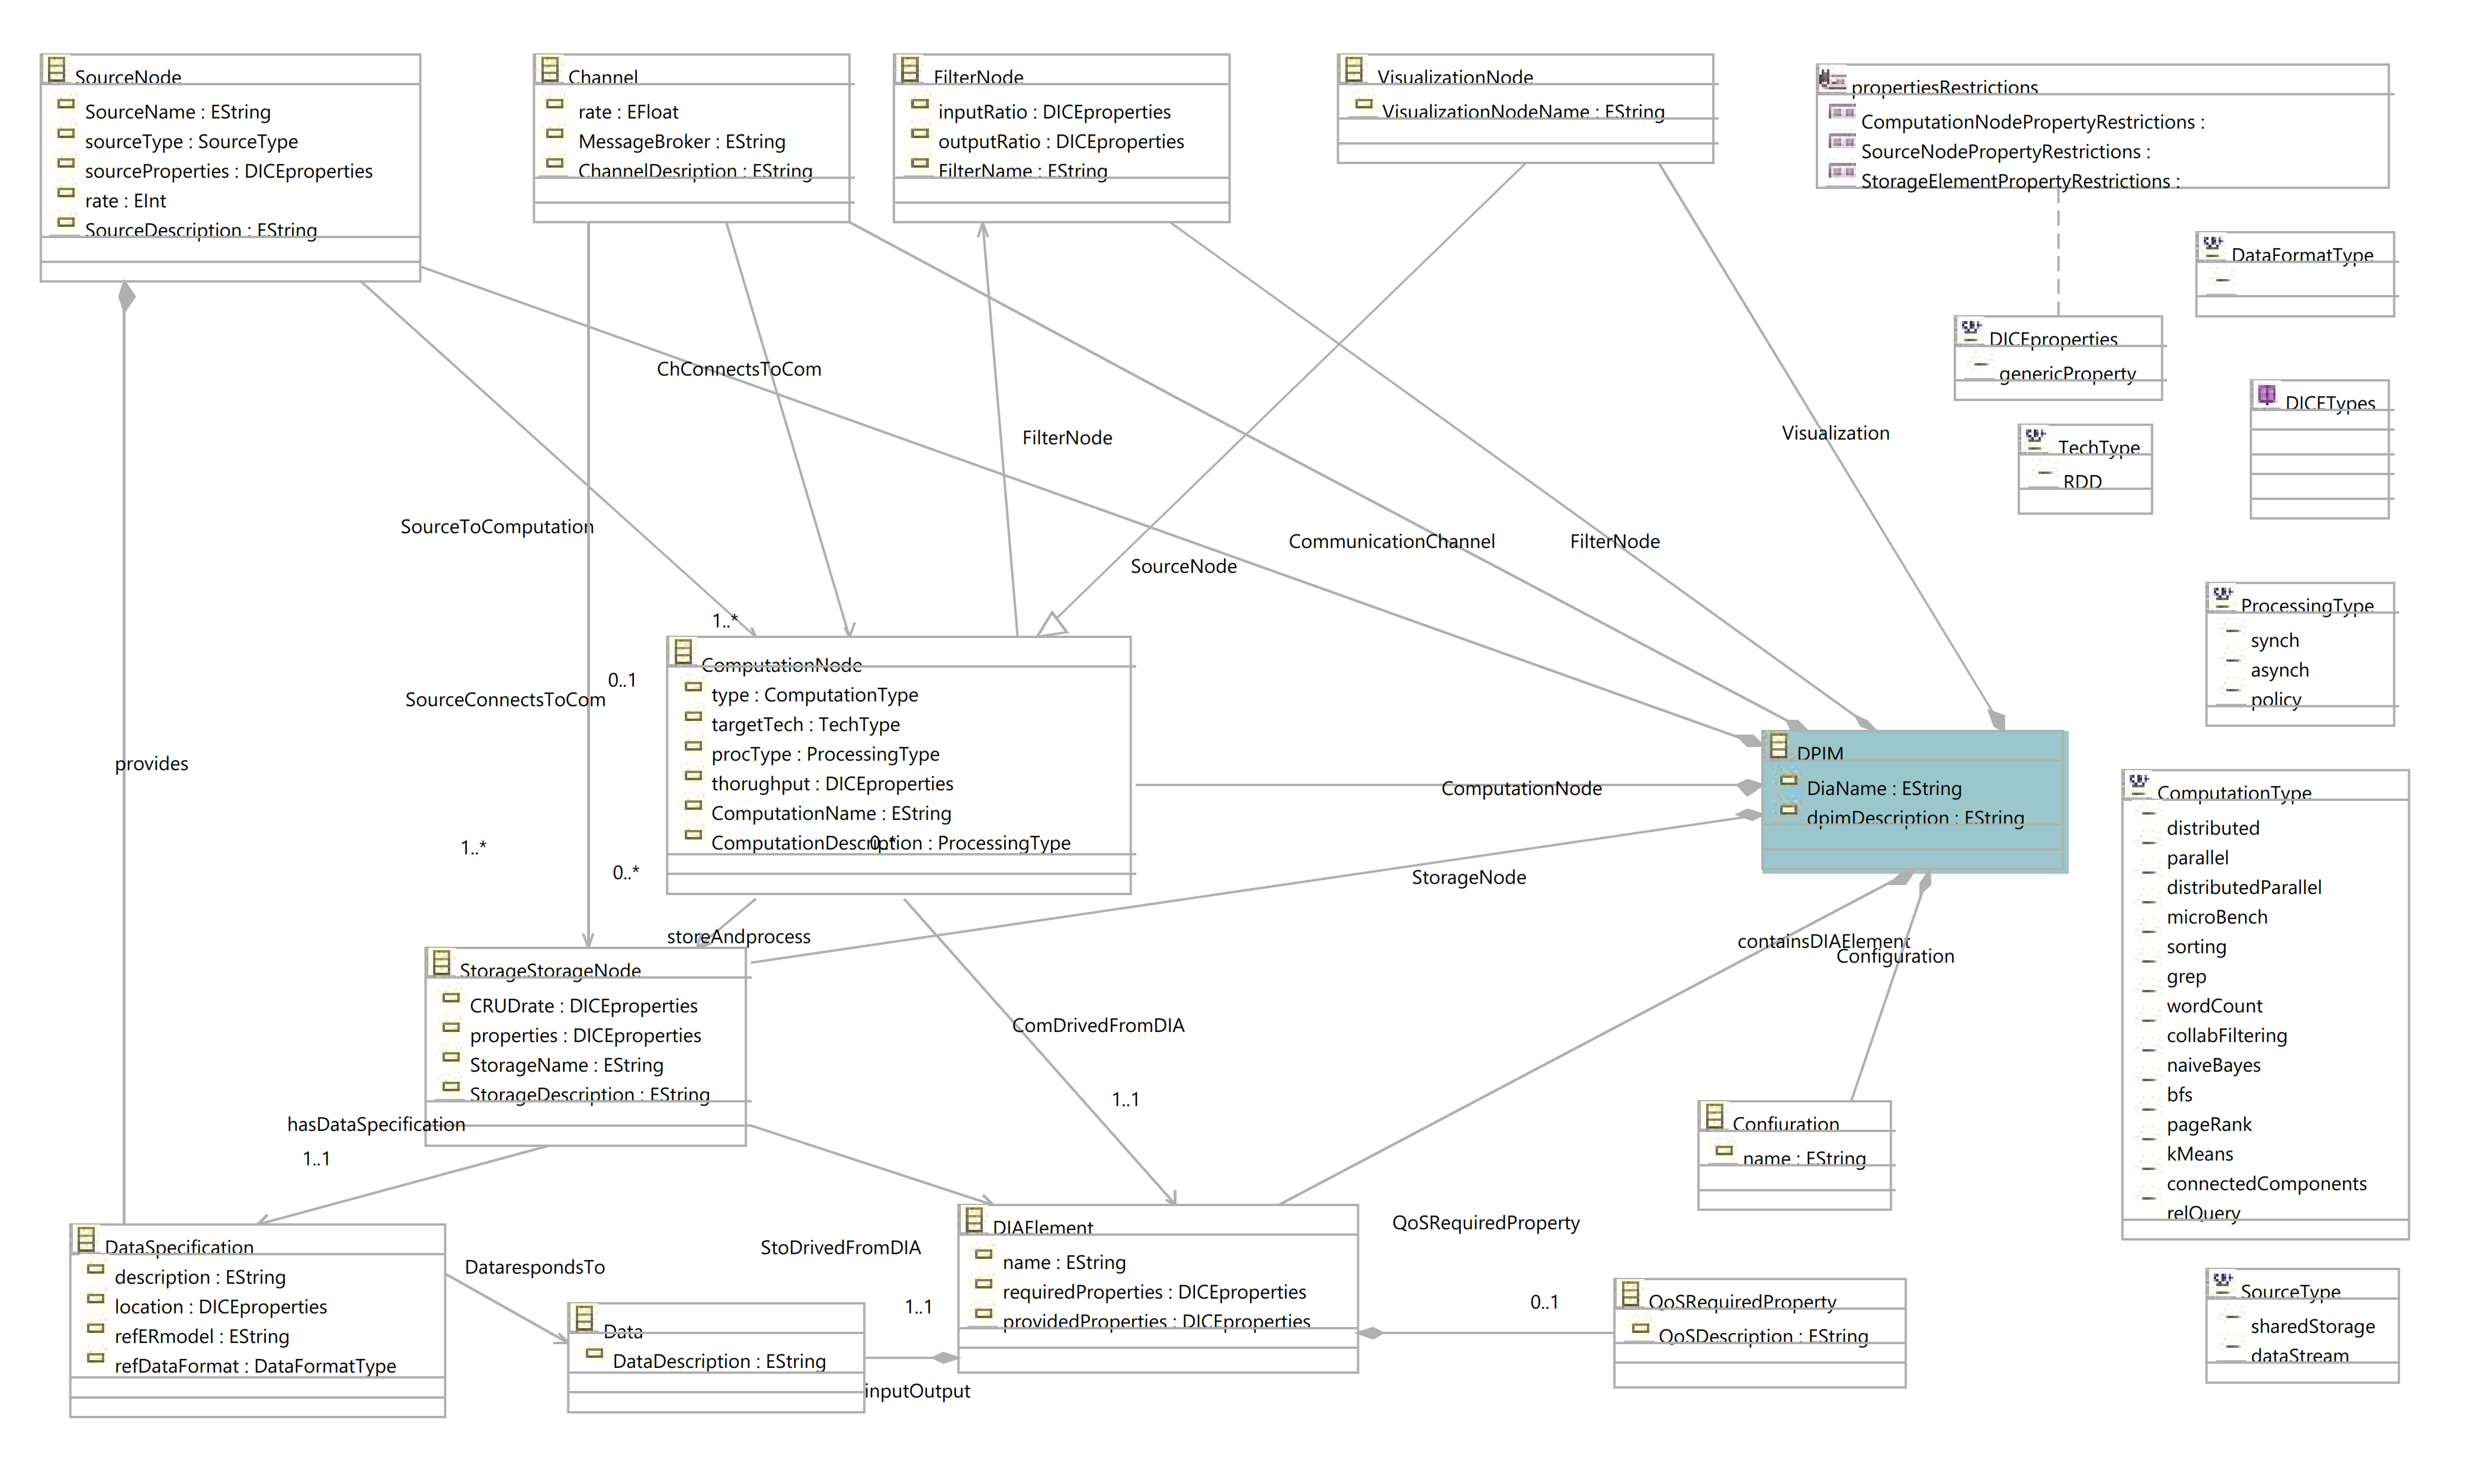
\includegraphics[width=\textwidth]{Images/11.png}
\caption{\label{fig:metamodel}DICE DPIM metamodel.}
\end{sidewaysfigure}

\begin{figure}
\centering
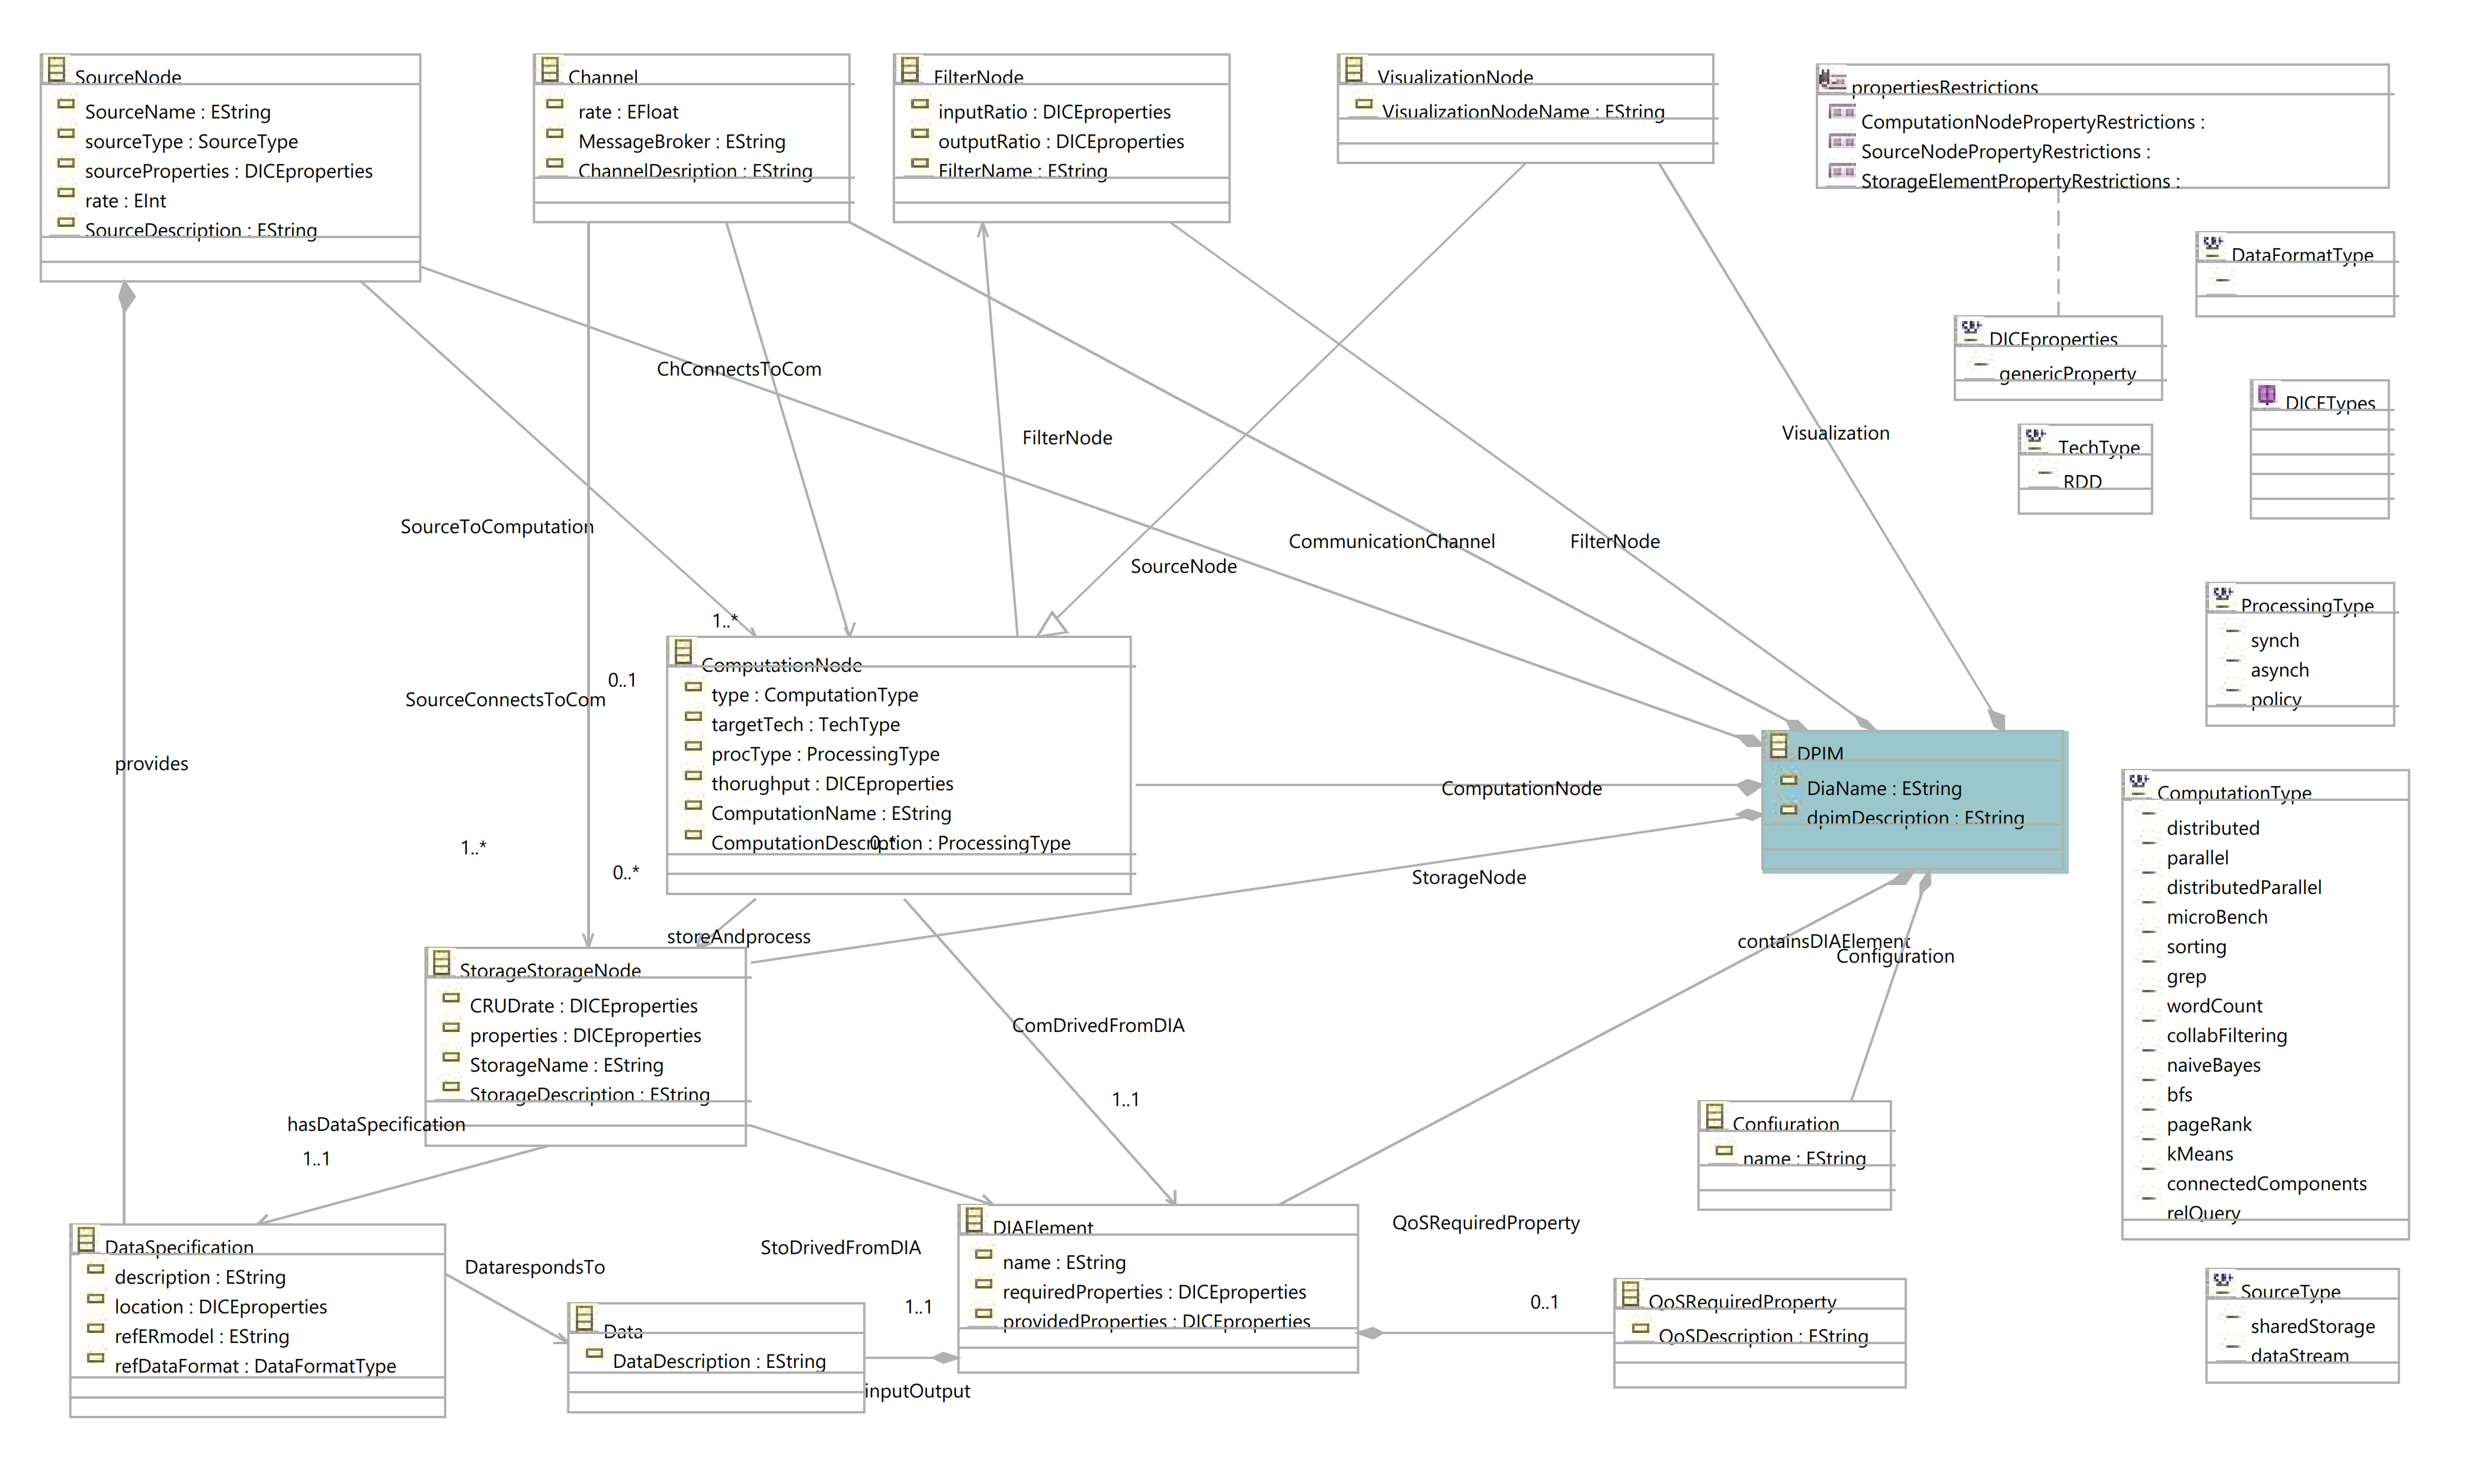
\includegraphics[width=\textwidth]{Images/11.png}
\caption{\label{fig:metamodel2}DICE DPIM metamodel in portrait form.}
\end{figure}

Here is the command to refer to another element (section, figure, table, ...) in the document: \emph{As discussed in Section~\ref{sect:overview} and as shown in Figure~\ref{fig:metamodel}, ...}. Here is how to introduce a bibliographic citation~\cite{DAM}. Bibliographic references should be included in a \texttt{.bib} file. 

Table generation is a bit complicated in Latex. You will soon become proficient, but to start you can rely on tools or external services. See for instance this \href{https://www.tablesgenerator.com}{https://www.tablesgenerator.com}. 


\clearpage
{\color{Blue}{\section{Specific Requirements}}}
\label{sect:requirements}
Organize this section according to the rules defined in the project description. 


\clearpage
{\color{Blue}{\section{Formal Analysis Using Alloy}}}
\label{sect:alloy}
This section describes the entire model formally using the alloy language.
In particular, we aim to model the relationships between entities that are used in the management of internships, such as students, companies and universities. Furthermore, we aim to ensure consistency by introducing the constraints that enable the creation and management of all processes in the system


\section{Alloy Code}
\lstinputlisting[language=alloy]{alloy/model.als}
\pagebreak

\section{Models}
\begin{enumerate}[label=,leftmargin=0cm]
      \item \textbf{Student participates in an internship}

            This model was generated using:
            \begin{lstlisting}[language=alloy]
            run {
                #Student = 2
	        #Company = 1
	        #Internship = 1
	        some i: Internship | i.state = InProgress
	        #Preferences >= 4
            } for 10
	
          \end{lstlisting}

            \begin{adjustbox}{max size={\textwidth}{\textheight}}
                  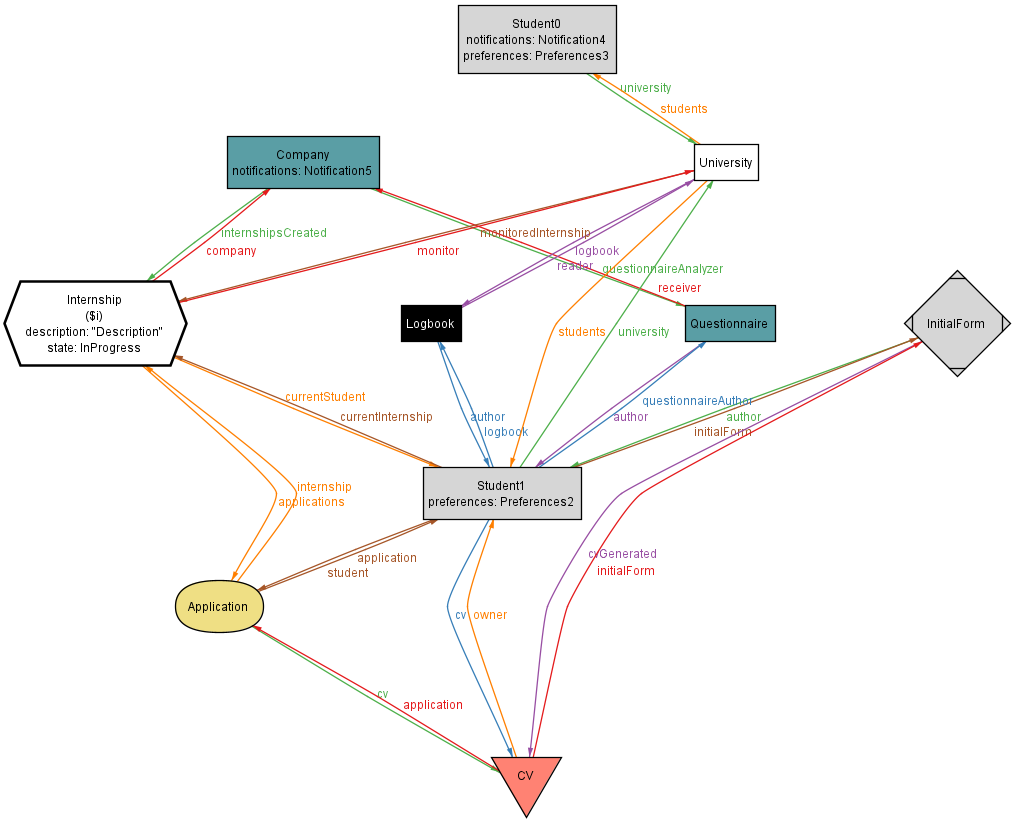
\includegraphics{alloy/alloy1.png}
            \end{adjustbox}

            This diagram shows us 2 students belonging to the same university. One of the two students is doing an internship at a company, and it shows us that this student had to fill out an ‘Initial Form’ in order to produce the CV that was used to make the application. The student also had to fill in a questionnaire at the selection stage and now has a logbook where he notes what he does in the company.

        \pagebreak
        \item \textbf{Company makes a report}

            This model was generated using:
            \begin{lstlisting}[language=alloy]
            run {
	        #Student = 3
	        #Company = 3
                #Internship = 3
                some i: Internship | i.state = InProgress
                #Preferences >= 4
                #ChatMessage >= 1
                #Report = 1
            } for 10
	
          \end{lstlisting}

            \begin{adjustbox}{max size={\textwidth}{\textheight}}
                  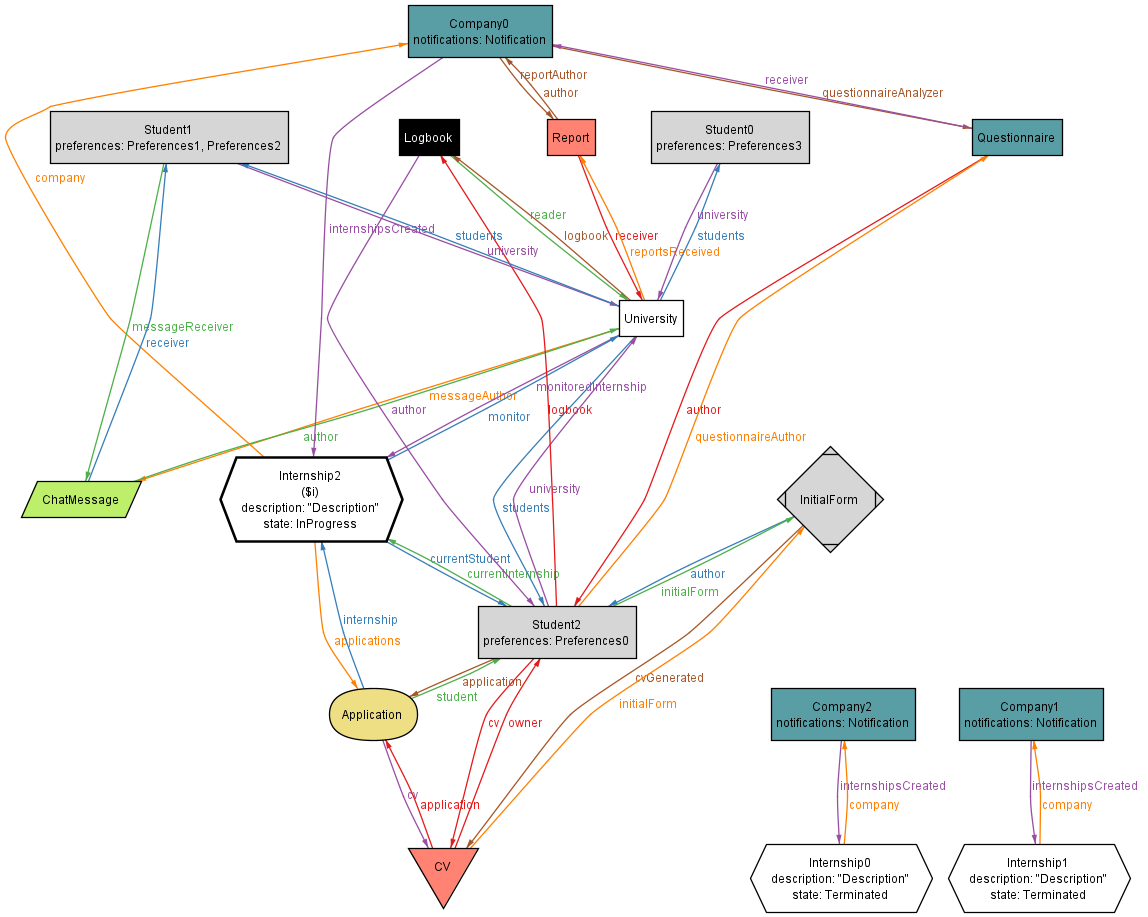
\includegraphics{RASD/alloy/alloy2.png}
            \end{adjustbox}

            This diagram shows us Student2 doing the Internship2, and he has in fact filled in an InitialForm and made the application (thus generating a CV). We also see that Company0, responsible for Internship2 has made a report to the university, probably reporting insufficient work by the student. We also see that Student1 has communicated with his university via chat. Finally, we can see that 2 other companies have created 2 internships which are now both terminated and therefore no longer have students
\end{enumerate}

\clearpage
{\color{Blue}{\section{Effort Spent}}}
\label{sect:effort}
Provide here information about how much effort each group member spent in working at this document. We would appreciate details here.


\clearpage
\addcontentsline{toc}{section}{References}
\bibliographystyle{plain}
\bibliography{main}

\end{document}